\chapter{Análisis}

La ingeniería de requisitos proporciona el mecanismo apropiado para entender lo que dice el cliente, analizar las necesidades, evaluar la factibilidad, negociar una solución, especificar la solución sin ambigüedades, validar la especificación y administrar los requisitos a medida que se transforman en un sistema funcional\cite{pressman}.

\section{Casos de uso}
Para poder entender cómo los usuarios emplearán finalmente las funciones y características del software, se debe crear un conjunto de escenarios que identifiquen la naturaleza de los usos para el sistema que se va a construir. La descripción de la manera en la que se utilizará el sistema se la conoce como caso de uso.

\subsection{Diagrama de casos de uso}
Las relaciones entre los actores y los casos de uso viene dada por el diagrama de casos de uso \ref{fig:diag_casos_uso}.

\begin{figure}[htbp] 
    \centering
    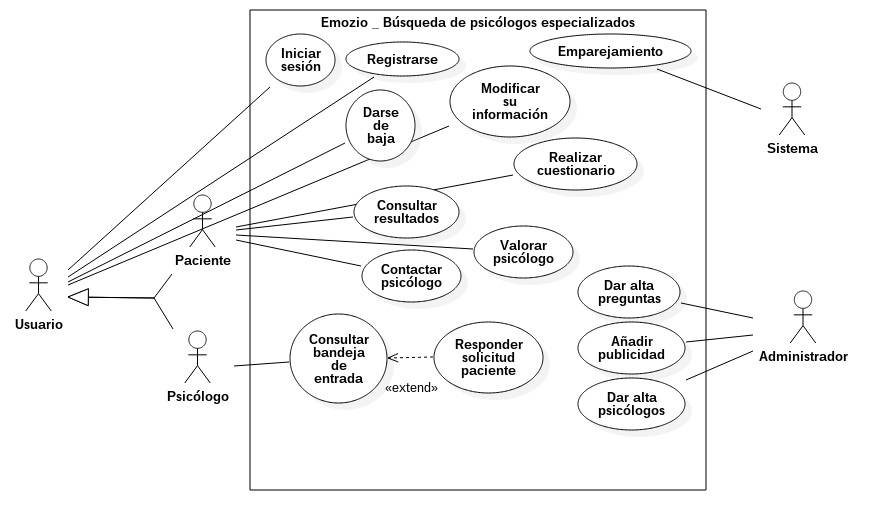
\includegraphics[width=1\textwidth]{figuras/diag_casos_uso.png}
    \caption{Diagrama de casos de uso}
    \label{fig:diag_casos_uso}
\end{figure}	

\subsection{Actores del sistema}
Un actor\ref{tab_actores} es cualquier cosa que se comunica con el sistema o producto y que sea externo a este. 

\begin{table}[htpb]
\centering
\begin{tabularx}{\textwidth}{|l|X|X|}
\hline
\multicolumn{1}{|c|}{\textbf{Identificador}} & \multicolumn{1}{c|}{\textbf{Nombre}} & \multicolumn{1}{c|}{\textbf{Descripción}}                                 \\ \hline
ACT-001                             & Usuario                     & Cualquier persona que acceda a nuestra plataforma web.           \\ \hline
ACT-002                             & Paciente                    & Cualquier persona que desee ser evaluada por nuestra aplicación. \\ \hline
ACT-003                             & Psicólogo                   & Cualquier persona que ejerza profesionalmente como psicólogo.    \\ \hline
ACT-004                             & Sistema                     & Encargado de ejecutar el algoritmo de emparejamiento.            \\ \hline
ACT-005                             & Administrador               & Persona encargada de gestionar los recursos de la aplicación.    \\ \hline
\end{tabularx}
\caption{Actores del sistema}
\label{tab_actores}
\end{table}


\subsection{Especificación de casos de uso}
Para poder determinar y evaluar correctamente cada caso de uso, tenemos una escala de la frecuencia de uso\ref{tab_frec_uso} y otra de la prioridad\ref{tab_prior}.

\begin{table}[htpb]
\centering
\begin{tabularx}{\textwidth}{|l|X|}
\hline
\multicolumn{2}{|c|}{\textbf{Frecuencia de uso}}                                                   \\ \hline
Ocasionalmente & Se utilizará en algunas ocasiones, no de forma habitual o por costumbre. \\ \hline
Puntualmente   & Se utilizará en raras ocasiones.                                         \\ \hline
Limitada       & Sólo podrá utilizarse en una única ocasión.                              \\ \hline
\end{tabularx}
\caption{Frecuencias de uso}
\label{tab_frec_uso}
\end{table}

\begin{table}[htpb]
\centering
\begin{tabularx}{\textwidth}{|l|X|}
\hline
\multicolumn{2}{|c|}{\textbf{Prioridad}}                                                                          \\ \hline
Alta  & El caso de uso es imprescindible para el funcionamiento normal de la aplicación.                 \\ \hline
Media & El caso de uso aporta funcionalidad necesaria en el sistema pero no aporta un valor fundamental. \\ \hline
Baja  & El caso de uso aporta funcionalidades extra pero es totalmente prescindible.                     \\ \hline
\end{tabularx}
\caption{Prioridades}
\label{tab_prior}
\end{table}

%
%CU-001
%
%
\begin{table}[htpb]
\centering
\begin{tabularx}{\textwidth}{|l|X|}
\hline
\textbf{CU-001}                            & \textbf{Iniciar sesión                                                                                                                                                                                                                                  } \\ \hline
Actor principal                   & Usuario                                                                                                                                                                                                                                          \\ \hline
Objetivo en contexto              & El usuario desea acceder a una cuenta de usuario ya existente mediante sus claves de acceso.                                                                                                                                                       \\ \hline
Precondiciones                    & Las claves de usuario deben ser válidas.                                                                                                                                                                                                         \\ \hline
Disparador                        & El usuario desea acceder a la plataforma para disfrutar de sus servicios.                                                                                                                                                                          \\ \hline
Escenario                         & \begin{tabular}{p{0.5cm} p{6cm}}1. & El usuario accede a Emozio.\\ 2. & El usuario introduce sus claves de acceso.\\ 3. & El usuario pulsa el botón de acceso.\\ 4. & El sistema muestra el perfil del usuario donde podrá acceder al resto de servicios.\end{tabular} \\ \hline
Excepciones                       & \begin{tabular}{p{0.5cm} p{6cm}}1. & Las claves de usuario son incorrectas.\\ 2. & El usuario no estaba registrado en la plataforma en el momento que se realizó el acceso.\end{tabular}                                                                    \\ \hline
Prioridad                         & Alta. El usuario debe iniciar sesión en la aplicación para poder utilizar cualquiera de sus servicios.                                                                                                                                             \\ \hline
Disponibilidad                    & En el segundo incremento                                                                                                                                                                                                                         \\ \hline
Frecuencia de uso                 & Ocasionalmente                                                                                                                                                                                                                                   \\ \hline
Canal del actor                   & A través de un navegador con acceso a Internet.                                                                                                                                                                                                  \\ \hline
Dependencias (con los requisitos) & \begin{tabular}[c]{@{}l@{}}RI-001\\ RI-003\\ RF-001\end{tabular}                                                                                                                                                                                 \\ \hline
\end{tabularx}
\caption{CU-001 Iniciar sesión}
%\label{my-label}
\end{table}

%%
%%CU-002
%%

\begin{table}[htpb]
\centering
\begin{tabularx}{\textwidth}{|l|X|}
\hline
\textbf{CU-002}                            & \textbf{Registrarse}                                                                                                                                                                                                                                                                                                                                                                                                                    \\ \hline
Actor principal                   & Paciente                                                                                                                                                                                                                                                                                                                                                                                                                        \\ \hline
Objetivo en contexto              & El paciente desea registrarse en la plataforma cediendo sus datos personales para poder acceder a los servicios de la plataforma.                                                                                                                                                                                                                                                                                                 \\ \hline
Precondiciones                    & Los datos introducidos en el formulario deben ser válidos.                                                                                                                                                                                                                                                                                                                                                                     \\ \hline
Disparador                        & El paciente desea registrarse en la plataforma para disfrutar de sus servicios.                                                                                                                                                                                                                                                                                                                                                   \\ \hline
Escenario                         & \begin{tabular}{p{0.5cm} p{6cm}} 1. & El paciente accede a Emozio. \\ 2. & El paciente introduce sus datos en un formulario de registro.\\ 3. & El paciente pulsa el botón de registro.\\ 4. & Se completa el registro.\\ 5. & El sistema muestra el perfil del usuario donde podrá acceder al resto de servicios. \end{tabular} \\ \hline
Excepciones                       & \begin{tabular}{p{0.5cm} p{6cm}}1. & Los datos introducidos en el formulario son incorrectos.\\ 2. & Ya existe el usuario dentro de la plataforma.\end{tabular}                                                                                                                                                                                                                                                                         \\ \hline
Prioridad                         & Alta. El paciente debe estar registrado en la aplicación para poder utilizar cualquiera de sus servicios.                                                                                                                                                                                                                                                                                                                         \\ \hline
Disponibilidad                    & En el segundo incremento                                                                                                                                                                                                                                                                                                                                                                                                       \\ \hline
Frecuencia de uso                 & Limitada                                                                                                                                                                                                                                                                                                                                                                                                                       \\ \hline
Canal del actor                   & A través de un navegador con acceso a internet.                                                                                                                                                                                                                                                                                                                                                                                \\ \hline
Dependencias (con los requisitos) & \begin{tabular}[c]{@{}l@{}}RI-001\\ RI-003\\ RF-001\\ RF-002\end{tabular}                                                                                                                                                                                                                                                                                                                                                      \\ \hline
\end{tabularx}
\caption{CU-002 Registrarse}
%\label{my-label}
\end{table}

%%
%%CU-003
%%

\begin{table}[htpb]
\centering
\begin{tabularx}{\textwidth}{|X|X|}
\hline
\textbf{CU-003}                            & \textbf{Realizar cuestionario                                                                                                                                                                                                                                                                                                                                                                                                                                                                                                   } \\ \hline
Actor principal                   & Paciente                                                                                                                                                                                                                                                                                                                                                                                                                                                                                                                 \\ \hline
Objetivo en contexto              & El paciente desea conocer qué profesional es el más adecuado para tratar su dolencia realizando el cuestionario de emparejamiento.                                                                                                                                                                                                                                                                                                                                                                                       \\ \hline
Precondiciones                    & El cuestionario debe estar cubierto.                                                                                                                                                                                                                                                                                                                                                                                                                                                                                     \\ \hline
Disparador                        & El paciente debe haber pulsado el botón de ``hacer el cuestionario''.                                                                                                                                                                                                                                                                                                                                                                                                                                                      \\ \hline
Escenario                         & \begin{tabular} {p{0.5cm} p{5cm}} 1. & El  paciente accede a Emozio.\\ 2. & El paciente entra en su perfil de usuario ya sea por registro o acceso.\\  3. & El sistema le muestra su perfil de usuario.\\ 4. & El paciente pulsa el botón de hacer el cuestionario.\\ 5. & El sistema le muestra el formulario que debe cubrir.\\ 6. & El paciente cubre las respuestas del formulario.\\ 7. & El paciente pulsa el botón de conocerlos resultados.\\ 8. & El sistema le mostrará su perfil en el que se encuentran los resultados.\end{tabular} \\ \hline
Excepciones                       & Los datos introducidos en el formulario son incorrectos.                                                                                                                                                                                                                                                                                                                                                                                                                                                                 \\ \hline
Prioridad                         & Alta. Es la característica central de la plataforma.                                                                                                                                                                                                                                                                                                                                                                                                                                                                     \\ \hline
Disponibilidad                    & En el primer incremento                                                                                                                                                                                                                                                                                                                                                                                                                                                                                                  \\ \hline
Frecuencia de uso                 & Puntualmente                                                                                                                                                                                                                                                                                                                                                                                                                                                                                                             \\ \hline
Canal del actor                   & A través de un navegador con acceso a Internet.                                                                                                                                                                                                                                                                                                                                                                                                                                                                          \\ \hline
Dependencias (con los requisitos) & \begin{tabular}[c]{@{}l@{}}RI-001\\ RI-002\\ RI-003\\ RF-001\\ RF-002\\  RF-005\end{tabular}                                                                                                                                                                                                                                                                                                                                                                                                                                       \\ \hline
\end{tabularx}
\caption{CU-003 Realizar cuestionario}
%\label{my-label}
\end{table}

%%
%%CU-004
%%

\begin{table}[htpb]
\centering
\begin{tabularx}{\textwidth}{|X|X|}
\hline
\textbf{CU-004}                            & \textbf{Consultar resultados}                                                                                                                                                                                                                                                     \\ \hline
Actor principal                   & Paciente                                                                                                                                                                                                                                                                 \\ \hline
Objetivo en contexto              & El paciente desea consultar el resultado del cuestionario de asignación.                                                                                                                                                                                                 \\ \hline
Precondiciones                    & El cuestionario debe estar cubierto.                                                                                                                                                                                                                                     \\ \hline
Disparador                        & El paciente debe acceder a su perfil.                                                                                                                                                                                                                                    \\ \hline
Escenario                         & \begin{tabular}{p{0.5cm} p{5cm}} 1. & El paciente accede a Emozio. \\ 2. & El paciente entra en su perfil de usuario ya sea por registro o acceso.\\ 3. & El sistema le muestra su perfil de usuario donde se encuentran los resultados del cuestionario de asignación.\end{tabular} \\ \hline
Excepciones                       & El paciente no ha cubierto el test en ninguna ocasión.                                                                                                                                                                                                                   \\ \hline
Prioridad                         & Alta. Es la característica central de la plataforma.                                                                                                                                                                                                                     \\ \hline
Disponibilidad                    & En el primer incremento                                                                                                                                                                                                                                                  \\ \hline
Frecuencia de uso                 & Ocasionalmente                                                                                                                                                                                                                                                           \\ \hline
Canal del actor                   & A través de un navegador con acceso a Internet.                                                                                                                                                                                                                          \\ \hline
Dependencias (con los requisitos) & \begin{tabular}[c]{@{}l@{}}RI-001\\ RI-003\\ RF-001\\ RF-002\\ RF-005\\ RF-006\end{tabular}                                                                                                                                                                                       \\ \hline
\end{tabularx}
\caption{CU-004 Consultar resultados}
%\label{my-label}
\end{table}

%%
%%CU-005
%%

\begin{table}[htpb]
\centering
\begin{tabularx}{\textwidth}{|X|X|}
\hline
\textbf{CU-005}                            & \textbf{Contactar psicólogo}                                                                                                                                                                                                                                                                                                                                                                                                                                                                                                                                                                                                                                                                                                        \\ \hline
Actor principal                   & Paciente                                                                                                                                                                                                                                                                                                                                                                                                                                                                                                                                                                                                                                                                                                                   \\ \hline
Objetivo en contexto              & El paciente desea ponerse en contacto con uno de los psicólogos que le han sido asignados.                                                                                                                                                                                                                                                                                                                                                                                                                                                                                                                                                                                                                                 \\ \hline
Precondiciones                    & \begin{tabular}{p{0.5cm} p{5cm}}1.  &  El cuestionario debe estar cubierto.\\ 2.  &  Las respuestas del cuestionario no dieron resultados imprecisos.\end{tabular}                                                                                                                                                                                                                                                                                                                                                                                                                                                                                                                                \\ \hline
Disparador                        & El paciente  accede a su perfil y se decide a contactar con el psicólogo.                                                                                                                                                                                                                                                                                                                                                                                                                                                                                                                                                                                                                                                  \\ \hline
Escenario                         & \begin{tabular}{p{0.5cm} p{5cm}}1.  &  El  paciente accede a Emozio.\\ 2.  &  El paciente entra en su perfil de usuario ya sea por registro o acceso.\\ 3.  &  El sistema le muestra su perfil de usuario donde se encuentran los resultados del cuestionario de asignación.\\ 4.  &  El paciente pulsa el botón de contacto del psicólogo en cuestión.\\ 5.  &  El sistema le muestra un formulario de contacto que debe cubrir.\\ 6.  &  El paciente cubre el formulario.\\ 7.  &  El paciente pulsa el botón de enviar.\\ 8.  &  El sistema muestra un mensaje con el estado de la operación.\end{tabular} \\ \hline
Excepciones                       & \begin{tabular}{p{0.5cm} p{5cm}}1.  &  El paciente no ha cubierto el test en ninguna ocasión.\\ 2.  &  El test dió un resultado impreciso para las respuestas dadas en el cuestionario.\end{tabular}                                                                                                                                                                                                                                                                                                                                                                                                                                                                                              \\ \hline
\end{tabularx}
\caption{CU-005 Contactar psicólogo - Parte 1}                                                                                                                                                                                                                                                                                                                                                                                                                                                                                                                                                                                                                                                                                                 
%\label{my-label}
\end{table}

\begin{table}[htpb]
\centering
\begin{tabularx}{\textwidth}{|X|X|}
\hline
\textbf{CU-005}                            & \textbf{Contactar psicólogo}                                                                                                                                                                                                                                                                                                                                                                                                                                                                                                                                                                                                                                                                                                        \\ \hline
Prioridad                         & Moderada. Puede implementarse después de las funciones básicas.                                                                                                                                                                                                                                                                                                                                                                                                                                                                                                                                                                                                                                                            \\ \hline
Disponibilidad                    & En el tercer incremento                                                                                                                                                                                                                                                                                                                                                                                                                                                                                                                                                                                                                                                                                                    \\ \hline
Frecuencia de uso                 & Puntualmente                                                                                                                                                                                                                                                                                                                                                                                                                                                                                                                                                                                                                                                                                                               \\ \hline
Canal del actor                   & A través de un navegador con acceso a Internet.                                                                                                                                                                                                                                                                                                                                                                                                                                                                                                                                                                                                                                                                            \\ \hline
Dependencias (con los requisitos) & \begin{tabular}[c]{@{}l@{}}RI-001\\ RI-003\\ RF-001\\ RF-002\\ RF-005\end{tabular}                                                                                                                                                                                                                                                                                                                                                                                                                                                                                                                                                                                             \\ \hline
\end{tabularx}
\caption{CU-005 Contactar psicólogo - Parte 2}                                                                                                                                                                                                                                                                                                                                                                                                                                                                                                                                                                                                                                                                                                 
%\label{my-label}
\end{table}

%%
%%CU-006
%%

\begin{table}[htpb]
\centering
\begin{tabularx}{\textwidth}{|X|X|}
\hline
\textbf{CU-006}                            & \textbf{Modificar información}                                                                                                                                                                                                                                                                                                                                                                                                                                                                                \\ \hline
Actor principal                   & Paciente                                                                                                                                                                                                                                                                                                                                                                                                                                                                                             \\ \hline
Objetivo en contexto              & El paciente desea cambiar sus datos porque en ese instante su información de usuario es incorrecta.                                                                                                                                                                                                                                                                                                                                                                                                   \\ \hline
Precondiciones                    & El paciente tiene acceso a la plataforma.                                                                                                                                                                                                                                                                                                                                                                                                                                                             \\ \hline
Disparador                        & El paciente debe acceder a su página principal.                                                                                                                                                                                                                                                                                                                                                                                                                                                       \\ \hline
Escenario                         & \begin{tabular}{p{0.5cm} p{5cm}}1. & El paciente accede a Emozio.\\ 2. & El paciente entra en su página principal ya sea por registro o acceso.\\ 3. & El sistema le muestra su página principal.\\ 4. & El paciente pulsa el botón de modificación de datos.\\ 5. & El sistema le muestra un formulario con sus datos actuales.\\ 6. & El paciente cubre el formulario con los datos correctos.\\ 7. & El paciente pulsa el botón de enviar.\\ 8. & El sistema le devolverá un mensaje de éxito. \end{tabular} \\ \hline
Excepciones                       & El paciente cancela la operación en curso.                                                                                                                                                                                                                                                                                                                                                                                                                                                            \\ \hline
Prioridad                         & Moderada. Puede implementarse después de las funciones básicas.                                                                                                                                                                                                                                                                                                                                                                                                                                      \\ \hline
Disponibilidad                    & En el segundo incremento                                                                                                                                                                                                                                                                                                                                                                                                                                                                             \\ \hline
Frecuencia de uso                 & Puntualmente                                                                                                                                                                                                                                                                                                                                                                                                                                                                                         \\ \hline
Canal del actor                   & A través de un navegador con acceso a Internet.                                                                                                                                                                                                                                                                                                                                                                                                                                                      \\ \hline
Dependencias (con los requisitos) & \begin{tabular}[c]{@{}l@{}}RI-001\\ RI-003\\ RF-001\\ RF-002\end{tabular}                                                                                                                                                                                                                                                                                                                                                                                                                            \\ \hline
\end{tabularx}
\caption{CU-006 Modificar información}                                                                                                                                                                                                                                                                                                                                                                                                                                                                           
%\label{my-label}
\end{table}

%%
%%CU-007
%%

\begin{table}[htpb]
\centering
\begin{tabularx}{\textwidth}{|X|X|}
\hline
\textbf{CU-007}                            & \textbf{Valorar psicólogo                                                                                                                                                                                                                                                                                                                                                                                                                                                                                                                                                                                                                                                                 } \\ \hline
Actor principal                   & Paciente                                                                                                                                                                                                                                                                                                                                                                                                                                                                                                                                                                                                                                                                           \\ \hline
Objetivo en contexto              & El paciente desea  valorar al psicólogo con el que se ha puesto en contacto.                                                                                                                                                                                                                                                                                                                                                                                                                                                                                                                                                                                                       \\ \hline
Precondiciones                    & El paciente se ha puesto en contacto previamente con el psicólogo en cuestión.                                                                                                                                                                                                                                                                                                                                                                                                                                                                                                                                                                                                     \\ \hline
Disparador                        & El paciente debe acceder al perfil del psicólogo.                                                                                                                                                                                                                                                                                                                                                                                                                                                                                                                                                                                                                                  \\ \hline
Escenario                         & \begin{tabular}{p{0.5cm} p{5cm}}1. & El  paciente accede a Emozio.\\ 2. & El paciente entra en su perfil de usuario ya sea por registro o acceso.\\ 3. & El sistema le muestra su perfil de usuario donde se encuentran los resultados del cuestionario de asignación.\\ 4. & El paciente pulsa el botón de mostrar más información del psicólogo.\\ 5. & El sistema le muestra el perfil del psicólogo seleccionado.\\ 6. & El paciente pulsa el botón de realizar valoración.\\ 7. & El sistema muestra un breve formulario que le permite valorar y escribir un mensaje.\\ 8. & El paciente pulsa el botón de enviar.\\ 9. & El sistema muestra un mensaje con el estado de la operación.\end{tabular} \\ \hline
Excepciones                       & \begin{tabular}{p{0.5cm} p{5cm}}1. & El paciente no se había puesto en contacto con el psicólogo previamente.\\ 2. & El paciente ya había dejado una valoración en el perfil del psicólogo.\end{tabular}                                                                                                                                                                                                                                                                                                                                                                                                                                                                                    \\ \hline
\end{tabularx}
\caption{CU-007 Valorar psicólogo - Parte 1}
%\label{my-label}
\end{table}

\begin{table}[htpb]
\centering
\begin{tabularx}{\textwidth}{|X|X|}
\hline
\textbf{CU-007}                            & \textbf{Valorar psicólogo}                                                                                                                                                                                                                                                                                                                                                                                                                                                                                                                                                                                                                                                                  \\ \hline
Prioridad                         & Moderada. Puede implementarse después de las funciones básicas.                                                                                                                                                                                                                                                                                                                                                                                                                                                                                                                                                                                                                    \\ \hline
Disponibilidad                    & En el tercer incremento                                                                                                                                                                                                                                                                                                                                                                                                                                                                                                                                                                                                                                                            \\ \hline
Frecuencia de uso                 & Puntualmente                                                                                                                                                                                                                                                                                                                                                                                                                                                                                                                                                                                                                                                                       \\ \hline
Canal del actor                   & A través de un navegador con acceso a Internet.                                                                                                                                                                                                                                                                                                                                                                                                                                                                                                                                                                                                                                    \\ \hline
Dependencias (con los requisitos) & \begin{tabular}[c]{@{}l@{}}RI-001\\ RI-002\\ RF-001\\ RF-002\\ RF-005\\ RF-007\end{tabular}                                                                                                                                                                                                                                                                                                                                                                                                                                                                                                                                                                                                 \\ \hline
\end{tabularx}
\caption{CU-007 Valorar psicólogo - Parte 2}
%\label{my-label}
\end{table}

%%
%%CU-008
%%

\begin{table}[htpb]
\centering
\begin{tabularx}{\textwidth}{|X|X|}
\hline
\textbf{CU-008}                            & \textbf{Filtrar resultados cuestionario}                                                                                                                                                                                                                                                                                                                                                                                                                                                               \\ \hline
Actor principal                   & Paciente                                                                                                                                                                                                                                                                                                                                                                                                                                                                                      \\ \hline
Objetivo en contexto              & El paciente desea filtrar su lista de psicólogos resultado en función de unos parámetros.                                                                                                                                                                                                                                                                                                                                                                                                     \\ \hline
Precondiciones                    & \begin{tabular}{p{0.5cm} p{5cm}}1. & El cuestionario debe estar cubierto.\\ 2. & Las respuestas del cuestionario no dieron resultados imprecisos.\end{tabular}                                                                                                                                                                                                                                                                                                                                         \\ \hline
Disparador                        & El paciente accede a su perfil y desea filtrar los resultados del cuestionario.                                                                                                                                                                                                                                                                                                                                                                                                               \\ \hline
Escenario                         & \begin{tabular}{p{0.5cm} p{5cm}}1. & El  paciente accede a Emozio.\\ 2. & El paciente entra en su perfil de usuario ya sea por registro o acceso.\\ 3. & El sistema le muestra su perfil de usuario donde se encuentran los resultados del cuestionario de asignación.\\ 4. & El paciente cubre el formulario de filtros que se muestra en la página.\\ 5. & El paciente pulsa el botón de enviar.\\ 6. & El sistema muestra el listado de resultados con los filtros que seleccionó el paciente.\end{tabular} \\ \hline
Excepciones                       & \begin{tabular}{p{0.5cm} p{5cm}}1. & El paciente no ha cubierto el test en ninguna ocasión.\\ 2. & El test dió un resultado impreciso para las respuestas dadas en el cuestionario.\end{tabular}                                                                                                                                                                                                                                                                                                       \\ \hline
Prioridad                         & Moderada. Puede implementarse después de las funciones básicas.                                                                                                                                                                                                                                                                                                                                                                                                                               \\ \hline
Disponibilidad                    & En el primer incremento                                                                                                                                                                                                                                                                                                                                                                                                                                                                       \\ \hline
Frecuencia de uso                 & Ocasionalmente                                                                                                                                                                                                                                                                                                                                                                                                                                                                                \\ \hline
Canal del actor                   & A través de un navegador con acceso a Internet.                                                                                                                                                                                                                                                                                                                                                                                                                                               \\ \hline
Dependencias (con los requisitos) & \begin{tabular}[c]{@{}l@{}}RI-001\\ RI-003\\ RF-001\\ RF-002\\ RF-005\end{tabular}                                                                                                                                                                                                                                                                                                                                                                                                                     \\ \hline
\end{tabularx}
\caption{CU-008 Filtrar resultados cuestionario}
%\label{my-label}
\end{table}

%%
%%CU-009
%%

\begin{table}[htpb]
\centering
\begin{tabularx}{\textwidth}{|X|X|}
\hline
\textbf{CU-009}                            & \textbf{Consultar perfil psicólogo}                                                                                                                                                                                                                                                                                                                                                                                          \\ \hline
Actor principal                   & Paciente                                                                                                                                                                                                                                                                                                                                                                                                            \\ \hline
Objetivo en contexto              & El paciente desea consultar la información de perfil de uno de los psicólogos resultado.                                                                                                                                                                                                                                                                                                                            \\ \hline
Precondiciones                    & \begin{tabular}{p{0.5cm} p{5cm}}1. & El cuestionario debe estar cubierto.\\ 2. & Las respuestas del cuestionario no dieron resultados imprecisos.\end{tabular}                                                                                                                                                                                                                                                               \\ \hline
Disparador                        & El paciente debe acceder al perfil del psicólogo.                                                                                                                                                                                                                                                                                                                                                                   \\ \hline
Escenario                         & \begin{tabular}{p{0.5cm} p{5cm}}1. & El  paciente accede a Emozio.\\ 2. & El paciente entra en su perfil de usuario ya sea por registro o acceso.\\ 3. & El sistema le muestra su perfil de usuario donde se encuentran los resultados del cuestionario de asignación.\\ 4. & El paciente pulsa el botón de mostrar más información del psicólogo.\\ 5. & El sistema le muestra el perfil del psicólogo seleccionado.\end{tabular} \\ \hline
Excepciones                       & El paciente cancela la operación en curso.                                                                                                                                                                                                                                                                                                                                                                          \\ \hline
Prioridad                         & Moderada. Puede implementarse después de las funciones básicas.                                                                                                                                                                                                                                                                                                                                                     \\ \hline
Disponibilidad                    & En el primer incremento                                                                                                                                                                                                                                                                                                                                                                                             \\ \hline
Frecuencia de uso                 & Ocasionalmente                                                                                                                                                                                                                                                                                                                                                                                                      \\ \hline
Canal del actor                   & A través de un navegador con acceso a internet.                                                                                                                                                                                                                                                                                                                                                                     \\ \hline
Dependencias (con los requisitos) & \begin{tabular}[c]{@{}l@{}}RI-001\\ RI-003\\ RF-001\\ RF-002\\ RF-005\end{tabular}                                                                                                                                                                                                                                                                                                                                           \\ \hline
\end{tabularx}
\caption{CU-009 Consultar perfil psicólogo}
%\label{my-label}
\end{table}

%%
%%CU-010
%%

\begin{table}[htpb]
\centering
\begin{tabularx}{\textwidth}{|X|X|}
\hline
\textbf{CU-010}                            & \textbf{Darse de baja}                                                                                                                                                                                                                                                                                                                                                                                                                                                                                                                                                                                                   \\ \hline
Actor principal                   & Usuario                                                                                                                                                                                                                                                                                                                                                                                                                                                                                                                                                                                                         \\ \hline
Objetivo en contexto              & El usuario desea darse debaja en la aplicación.                                                                                                                                                                                                                                                                                                                                                                                                                                                                                                                                                                 \\ \hline
Precondiciones                    & El usuario tiene acceso a la plataforma.                                                                                                                                                                                                                                                                                                                                                                                                                                                                                                                                                                        \\ \hline
Disparador                        & El usuario debe acceder a su página principal.                                                                                                                                                                                                                                                                                                                                                                                                                                                                                                                                                                  \\ \hline
Escenario                         & \begin{tabular}{p{0.5cm} p{5cm}}1. & El usuario accede a Emozio.\\ 2. & El usuario entra en su página principal ya sea por registro o acceso.\\ 3. & El sistema le muestra su página principal.\\ 4. & El usuario pulsa el botón de modificación de datos.\\ 5. & El sistema le muestra un formulario con sus datos actuales, y un botón para darse de baja.\\ 6. & El usuario pulsa el botón de darse de baja.\\ 7. & El sistema muestra un \textit{pop-up} pidiendo confirmación para ejecutar la operación.\\ 8. & El sistema elimina al usuario de la base de datos.\\ 9. & El sistema muestra al usuario la página de inicio.\end{tabular} \\ \hline
Excepciones                       & El usuario cancela la operación en curso.                                                                                                                                                                                                                                                                                                                                                                                                                                                                                                                                                                       \\ \hline
Prioridad                         & Moderada. Puede implementarse después de las funciones básicas.                                                                                                                                                                                                                                                                                                                                                                                                                                                                                                                                                 \\ \hline
Disponibilidad                    & En el segundo incremento                                                                                                                                                                                                                                                                                                                                                                                                                                                                                                                                                                                        \\ \hline
Frecuencia de uso                 & Limitada                                                                                                                                                                                                                                                                                                                                                                                                                                                                                                                                                                                                        \\ \hline
Canal del actor                   & A través de un navegador con acceso a Internet.                                                                                                                                                                                                                                                                                                                                                                                                                                                                                                                                                                 \\ \hline
Dependencias (con los requisitos) & \begin{tabular}[c]{@{}l@{}}RI-001\\ RI-003\\ RF-001\\ RF-002\end{tabular}                                                                                                                                                                                                                                                                                                                                                                                                                                                                                                                                                \\ \hline
\end{tabularx}
\caption{CU-010 Darse de baja}                                                                                                                                                                                                                                                                                                                                                                                                                                                                                                                                                                                                  
%\label{my-label}
\end{table}

%%
%%CU-011
%%

\begin{table}[htpb]
\centering
\begin{tabularx}{\textwidth}{|X|X|}
\hline
\textbf{CU-011}                            & \textbf{Consultar bandeja de entrada}                                                                                                                                                                           \\ \hline
Actor principal                   & Psicólogo                                                                                                                                                                                              \\ \hline
Objetivo en contexto              & El psicólogo desea consultar las peticiones que le han llegado a su bandeja de entrada.                                                                                                                \\ \hline
Precondiciones                    & Estar registrado.                                                                                                                                                                                      \\ \hline
Disparador                        & El psicólogo accede a su perfil y quiere consultar su bandeja de entrada.                                                                                                                              \\ \hline
Escenario                         & \begin{tabular}{p{0.5cm} p{5cm}}1. & El psicólogo accede a Emozio.\\ 2. & El psicólogo accede a su perfil de usuario.\\ 3. & El sistema le muestra los mensajes pendientes de su bandeja de entrada.\end{tabular} \\ \hline
Excepciones                       & -                                                                                                                                                                                                      \\ \hline
Prioridad                         & Moderada. Puede implementarse después de las funciones básicas.                                                                                                                                        \\ \hline
Disponibilidad                    & En el tercer incremento                                                                                                                                                                                \\ \hline
Frecuencia de uso                 & Ocasionalmente                                                                                                                                                                                         \\ \hline
Canal del actor                   & A través de un navegador con acceso a Internet.                                                                                                                                                        \\ \hline
Dependencias (con los requisitos) & \begin{tabular}[c]{@{}l@{}}RI-001\\ RI-003\\ RF-001\\ RF-002\end{tabular}                                                                                                                                       \\ \hline
\end{tabularx}
\caption{CU-011 Consultar bandeja de entrada}
%\label{my-label}
\end{table}

%%
%%CU-012
%%

\begin{table}[htpb]
\centering
\begin{tabularx}{\textwidth}{|X|X|}
\hline
\textbf{CU-012}                            & \textbf{Responder solicitud paciente                                                                                                                                                                                                                                                                                                                                               } \\ \hline
Actor principal                   & Psicólogo                                                                                                                                                                                                                                                                                                                                                                   \\ \hline
Objetivo en contexto              & El psicólogo desea responder a una de las peticiones que le han llegado a su bandeja de entrada.                                                                                                                                                                                                                                                                            \\ \hline
Precondiciones                    & Tener peticiones pendientes en la bandeja de entrada.                                                                                                                                                                                                                                                                                                                       \\ \hline
Disparador                        & El psicólogo accede a su perfil, consulta su bandeja de entrada y selecciona una de las peticiones.                                                                                                                                                                                                                                                                         \\ \hline
Escenario                         & \begin{tabular}{p{0.5cm} p{5cm}}1. & El psicólogo accede a Emozio.\\ 2. & El psicólogo accede a su perfil de usuario.\\ 3. & El sistema le muestra los mensajes pendientes de su bandeja de entrada.\\ 4. & El psicólogo selecciona una de las peticiones pendientes y la responde.\\ 5. & El sistema muestra un mensaje de éxito, y pasa la petición pendiente a respondida.\end{tabular} \\ \hline
Excepciones                       & -                                                                                                                                                                                                                                                                                                                                                                           \\ \hline
Prioridad                         & Moderada. Puede implementarse después de las funciones básicas.                                                                                                                                                                                                                                                                                                             \\ \hline
Disponibilidad                    & En el tercer incremento                                                                                                                                                                                                                                                                                                                                                     \\ \hline
Frecuencia de uso                 & Ocasionalmente                                                                                                                                                                                                                                                                                                                                                              \\ \hline
Canal del actor                   & A través de un navegador con acceso a Internet.                                                                                                                                                                                                                                                                                                                             \\ \hline
Dependencias (con los requisitos) & \begin{tabular}[c]{@{}l@{}}RI-001\\ RI-003\\ RF-001\\ RF-002\end{tabular}                                                                                                                                                                                                                                                                                                            \\ \hline
\end{tabularx}
\caption{CU-012 Responder solicitud paciente}
%\label{my-label}
\end{table}

\clearpage

%%
%%CU-013
%%

\begin{table}[htbp]
\centering
\begin{tabularx}{\textwidth}{|X|X|}
\hline
\textbf{CU-013}                            & \textbf{Emparejamiento                                                                                                            } \\ \hline
Actor principal                   & Sistema                                                                                                                    \\ \hline
Objetivo en contexto              & El sistema realiza el emparejamiento paciente-psicólogo.                                                                   \\ \hline
Precondiciones                    & El paciente en cuestión se disponga a realizar el test.                                                                    \\ \hline
Disparador                        & El paciente selecciona ``Hacer el test''.                                                                                    \\ \hline
Escenario                         & Cuando se envíen los resultados del test de un paciente, el sistema hará la correspondiente asignación paciente-psicólogo. \\ \hline
Excepciones                       & -                                                                                                                          \\ \hline
Prioridad                         & Alta. Es la característica central de la plataforma.                                                                       \\ \hline
Disponibilidad                    & En el primer incremento                                                                                                    \\ \hline
Frecuencia de uso                 & Ocasionalmente                                                                                                             \\ \hline
Canal del actor                   & A través de un navegador con acceso a Internet.                                                                            \\ \hline
Dependencias (con los requisitos) & \begin{tabular}[c]{@{}l@{}}RI-001\\ RI-003\\ RF-001\\ RF-002\\  RF-005\end{tabular}                                                  \\ \hline
\end{tabularx}
\caption{CU-013 Emparejamiento}                        
%\label{my-label}
\end{table}

\clearpage

%%
%%CU-014
%%

\begin{table}[htpb]
\centering
\begin{tabularx}{\textwidth}{|X|X|}
\hline
\textbf{CU-014}                            & \textbf{Dar alta a las preguntas}                                                                  \\ \hline
Actor principal                   & Administrador                                                                             \\ \hline
Objetivo en contexto              & El administrador dará de alta a las preguntas asociadas a las patologías.                 \\ \hline
Precondiciones                    & Tener nuevas preguntas para añadir al cuestionario.                                       \\ \hline
Disparador                        & Aparece una nueva patología o se modifican y/o actualizan las preguntas de una patología. \\ \hline
Escenario                         & El administrador añade las preguntas a la base de datos.                                  \\ \hline
Excepciones                       & -                                                                                         \\ \hline
Prioridad                         & Alta. Es la característica central de la plataforma.                                      \\ \hline
Disponibilidad                    & En el primer incremento                                                                   \\ \hline
Frecuencia de uso                 & Puntualmente                                                                              \\ \hline
Canal del actor                   & A través de una herramienta de gestión de bases de datos.                                 \\ \hline
Dependencias (con los requisitos) & RI-002                                                                                    \\ \hline
\end{tabularx}
\caption{CU-014 Dar alta a las preguntas}
%\label{my-label}
\end{table}

\clearpage

%%
%%CU-015
%%

\begin{table}[htpb]
\centering
\begin{tabularx}{\textwidth}{|X|X|}
\hline
\textbf{CU-015}                            & \textbf{Añadir la publicidad}                                                                           \\ \hline
Actor principal                   & Administrador                                                                                  \\ \hline
Objetivo en contexto              & El administrador añadirá la publicidad necesaria a la aplicación en el momento que se precise. \\ \hline
Precondiciones                    & -                                                                                              \\ \hline
Disparador                        & El administrador quiere actualizar los contenidos publicitarios.                               \\ \hline
Escenario                         & El administrador añade las preguntas a la base de datos.                                       \\ \hline
Excepciones                       & -                                                                                              \\ \hline
Prioridad                         & Moderada. Puede implementarse después de las funciones básicas.                                \\ \hline
Disponibilidad                    & En el tercer incremento                                                                        \\ \hline
Frecuencia de uso                 & Puntualmente                                                                                   \\ \hline
Canal del actor                   & A través de una herramienta de edición de código.                                              \\ \hline
Dependencias (con los requisitos) & -                                                                                              \\ \hline
\end{tabularx}
\caption{CU-015 Añadir la publicidad}                          
%\label{my-label}
\end{table}

\clearpage

%%
%%CU-016
%%

\begin{table}[htpb]
\centering
\begin{tabularx}{\textwidth}{|X|X|}
\hline
\textbf{CU-016}                            & \textbf{Dar alta psicólogos                                                                           } \\ \hline
Actor principal                   & Administrador                                                                                  \\ \hline
Objetivo en contexto              & El administrador dará de alta a los psicólogos que hayan enviado el formulario de registro.    \\ \hline
Precondiciones                    & El psicólogo que se va a dar de alta, ha de haber cubierto el formulario de registro.          \\ \hline
Disparador                        & El administrador desea actualizar la colección de psicólogos de la base de datos.              \\ \hline
Escenario                         & El administrador añade la información del psicólogo a la base de datos.                        \\ \hline
Excepciones                       & -                                                                                              \\ \hline
Prioridad                         & Moderada. Puede implementarse después de las funciones básicas.                                \\ \hline
Disponibilidad                    & En el segundo incremento                                                                       \\ \hline
Frecuencia de uso                 & Puntualmente                                                                                   \\ \hline
Canal del actor                   & A través de un navegador con acceso a Internet y una herramienta de gestión de bases de datos. \\ \hline
Dependencias (con los requisitos) & \begin{tabular}[c]{@{}l@{}}RI-003\\ RI-002\end{tabular}                                        \\ \hline
\end{tabularx}
\caption{CU-016 Dar alta psicólogos}                          
%\label{my-label}
\end{table}

\begin{table}[htpb]
\centering
\begin{tabularx}{\textwidth}{|X|X|}
\hline
\textbf{CU-017}                            & \textbf{Modificar la información de los psicólogos                                                                           } \\ \hline
Actor principal                   & Administrador                                                                                  \\ \hline
Objetivo en contexto              & El administrador modificará la información de los psicólogos que hayan enviado el formulario de modificación de datos.    \\ \hline
Precondiciones                    & El psicólogo ha de enviar el formulario cubierto.          \\ \hline
Disparador                        & El administrador desea actualizar la colección de psicólogos de la base de datos.              \\ \hline
Escenario                         & El administrador modifica la información del psicólogo a la base de datos.                        \\ \hline
Excepciones                       & -                                                                                              \\ \hline
Prioridad                         & Moderada. Puede implementarse después de las funciones básicas.                                \\ \hline
Disponibilidad                    & En el segundo incremento                                                                       \\ \hline
Frecuencia de uso                 & Puntualmente                                                                                   \\ \hline
Canal del actor                   & A través de un navegador con acceso a Internet y una herramienta de gestión de bases de datos. \\ \hline
Dependencias (con los requisitos) & \begin{tabular}[c]{@{}l@{}}RI-003\\ RI-002\end{tabular}                                        \\ \hline
\end{tabularx}
\caption{CU-017 Dar alta psicólogos}                          
%\label{my-label}
\end{table}

%%%%%%%%%%%%%%%%%%%%%%%%%%%%%%%%%%%%%%%%%%%%%%%%%%%%%%%%%%%%%%%%%%%%%%%%%%%%%%%%%%%%%%%
%%MODELO DE DATOS%%%%%%%%%%%%%%%%%%%%%%%%%%%%%%%%%%%%%%%%%%%%%%%%%%%%%%%%%%%%%%%%%%%%%%
%%%%%%%%%%%%%%%%%%%%%%%%%%%%%%%%%%%%%%%%%%%%%%%%%%%%%%%%%%%%%%%%%%%%%%%%%%%%%%%%%%%%%%%

\section{Modelado de datos}
Si los requisitos del \textit{software} incluyen la necesidad de crear, ampliar o hacer interfaz con una base de datos, o si deben construirse y manipularse estructuras de datos complejas, se debe crear un modelo de datos como parte del modelado general de los requisitos\cite{pressman}.


Los modelos semánticos de datos son la definición de la forma lógica de los datos procesados por el sistema\cite{sommerville}. 


\subsection{¿Por qué MongoDB?}
En nuestro proyecto, los datos se encuentran almacenados en una MongoDB que consiste en una base de datos NoSQL\footnote{Las bases de datos NoSQL son aquellas que generalmente no son relacionales y no tienen un lenguaje de consulta como SQL.} de código abierto, orientada a documentos y a mantener datos desestructurados, sobretodo cuando ésta crece exponencialmente\cite{mongodb_traspas}. 

\subsection{Comparativa MongoDB con SQL}
Teniendo de referencia una base de datos SQL podemos comprender cómo MongoDB almacena la información con una pequeña analogía. En la gestión de sistemas de bases de datos relacionales, los datos se guardan en filas contenidas dentro de tablas. En cambio, en MongoDB los datos son guardados como documentos contenidos en colecciones.


Una colección es un conjunto de documentos, como éstos son independientes, pueden contener distintos campos, lo que indica que su esquema es dinámico. A su vez, estos documentos son muy similares a los \textit{JSON Objects}, son conocidos como \textit{BSON objects} y la principal diferencia es que contienen a mayores el tipo \textit{ObjectID} que sirve de identificador del documento. Aquí es donde resaltamos una de las ventajas de utilizar MongoDB dentro de MEAN Stack, puesto que la información manejada en el lado cliente se obtiene y representa del mismo modo en el lado servidor.


En nuestro proyecto, las bases de datos son NoSQL, las cuales no tienen una representación estandarizada. Por tanto, y por entendimiento, se ha realizado a mayores una aproximación del modelo no relacional\ref{fig:mod_datos_mongoDB} al de un modelo entidad relación\ref{fig:mod_datos_mer}.

\subsection{Modelo de datos NoSQL}
En nuestro modelo de datos NoSQL la información está organizada en colecciones. Se debe resaltar que en algunas ocasiones, los documentos se encuentran embebidos dentro de otros. Como por ejemplo, en el caso de los comentarios de los psicólogos. Los comentarios son documentos embebidos (no tienen \textit{ObjectID}) dentro de los documentos de la colección de psicólogos.


Por otra parte, están los documentos referenciados, que son independientes. Tomando el mismo ejemplo anterior, dentro de un documento embebido de comentarios hayamos una referencia a un documento de la colección de pacientes (\texttt{\_idPaciente}).


La estructura se ha creado de este modo porque embebiendo documentos sólo se necesitaría una única consulta, el documento en cuestión se accedería con su documento padre y las escrituras serían atómicas (no se tendrían que escribir en múltiples documentos). Pero en el caso de que el documento sea de gran relevancia y obtenga gran cantidad de información, se hará referencia a él.


\begin{figure}[htbp] 
    \centering
    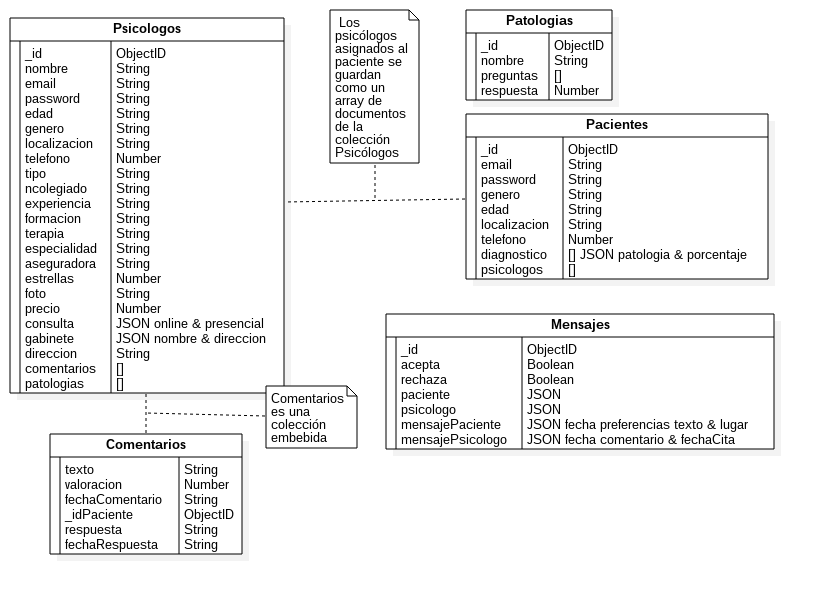
\includegraphics[width=1\textwidth]{figuras/bbdd_mod_mongoDB.png}
    \caption{Modelo de datos MongoDB}
    \label{fig:mod_datos_mongoDB}
\end{figure}	

\subsection{Modelo entidad-relación (MER)}
El modelo entidad-relación-atributo\ref{fig:mod_datos_mer} muestra las entidades de datos sus atributos asociados y las relaciones entre estas entidades. 


\begin{figure}[htbp] 
    \centering
    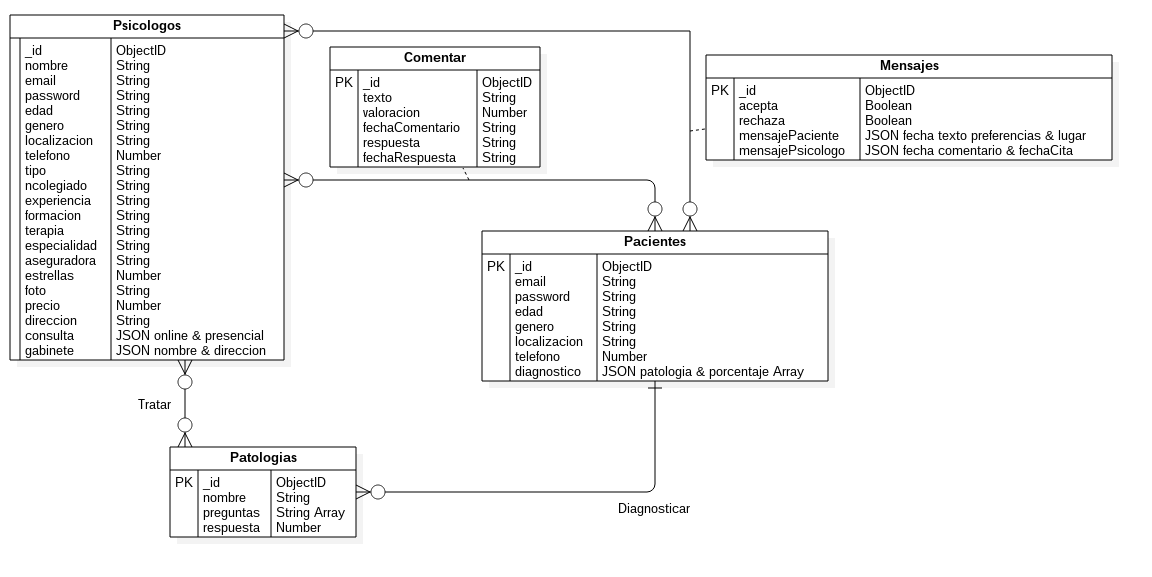
\includegraphics[width=1\textwidth]{figuras/bbdd_mod_MER.png}
    \caption{Modelo entidad-relación}
    \label{fig:mod_datos_mer}
\end{figure}

\subsection{Diccionario de datos}
Para mantener descripciones más detalladas de las entidades incluidas en el modelo se utilizan diccionarios de datos para gestionar toda la información.


Por tanto, un diccionario de datos es una lista de nombres ordenada alfabéticamente incluido en los modelos del sistema. Este nos proporciona un mecanismo de gestión e inventariado de nombres y sirve como un almacén de información.


Las colecciones vienen descritas en la tabla \ref{fig:dic_datos_colecciones}.

\begin{table}[htpb]
\centering
\begin{tabularx}{\textwidth}{|l|X|}
\hline
\textbf{Colección}  & \textbf{Descripción}                                                                               \\ \hline
Mensajes   & Almacena toda la información referente a las comunicaciones entre psicólogos y pacientes. \\ \hline
Pacientes  & Almacena toda la información sobre los pacientes del sistema.                             \\ \hline
Patologías & Almacena todas las patologías registradas hasta el momento en el sistema.                 \\ \hline
Psicólogos & Almacena toda la información sobre los psicólogos del sistema.                            \\ \hline
\end{tabularx}
\caption{Diccionario de datos: Colecciones}
\label{fig:dic_datos_colecciones}
\end{table}

Los objetos BSON de los documentos se pueden ver en las tablas \ref{fig:dic_datos_BSON_1},  \ref{fig:dic_datos_BSON_2}, \ref{fig:dic_datos_BSON_3} y \ref{fig:dic_datos_BSON_4}.

\begin{table}[htpb]
\centering
\begin{tabularx}{\textwidth}{|l|X|X|X|}
\hline
\multirow{2}{*}{\textbf{Documento}} & \multicolumn{3}{l|}{\textbf{Esquema BSON}}                                                                                                                                                                                                                                                                                                                               \\ \cline{2-4} 
                                    & \textbf{Campo}                                        & \textbf{Tipo de dato}                    & \textbf{Descripción}                                                                                                                                                                                                                                                  \\ \hline
\multirow{7}{*}{\textbf{Mensaje}}   & \_id                                                  & ObjectID                                 & Identificador del documento                                                                                                                                                                                                                                           \\ \cline{2-4} 
                                    & acepta                                                & Boolean                                  & El psicólogo acepta la solicitud de un paciente.                                                                                                                                                                                                                      \\ \cline{2-4} 
                                    & mensajePaciente \begin{itemize}
                                    \item consulta
                                    \item fecha
                                    \item preferencias
                                    \item texto
                                    \end{itemize} & JSON \begin{itemize}
                                    \item String
                                    \item String
                                    \item String
                                    \item String
                                    \end{itemize} & Es la información del mensaje que le envía un paciente al psicólogo. Se guarda la fecha donde fue enviado el mensaje, las preferencias horarias que tendría el paciente, el comentario que quiera transmitirle el paciente y dónde quiere que se realice la consulta. \\ \cline{2-4} 
                                    & paciente                                              & JSON                                     & Guarda información necesaria del documento del paciente que envió el mensaje.                                                                                                                                                                                         \\ \cline{2-4} 
                                    & psicólogo                                             & JSON                                     & Guarda información necesaria del documento del psicólogo que recibió el mensaje.                                                                                                                                                                                      \\ \cline{2-4} 
                                    & rechaza                                               & Boolean                                  & El psicólogo rechaza la solicitud de un paciente.                                                                                                                                                                                                                     \\ \cline{2-4} 
                                    & mensajePsicologo \begin{itemize}
                                    \item comentario
                                    \item fecha
                                    \item fechaCita
\end{itemize}                       & JSON \begin{itemize}
\item String 
\item String 
\item String 
\end{itemize}          & Mensaje que envía un psicólogo como respuesta a la solicitud de un paciente. Se guarda el comentario que quiera transmitirle el psicólogo, la fecha en que fué enviado el mensaje y la fecha de la cita en caso de que se la dé.                                      \\ \hline
\end{tabularx}
\caption{Diccionario de datos: BSON Documento Mensaje}
\label{fig:dic_datos_BSON_1}
\end{table}

\begin{table}[htpb]
\centering
\begin{tabularx}{\textwidth}{|l|X|X|X|X|}
\hline
\multirow{2}{*}{\textbf{Documento}} & \multicolumn{3}{l|}{\textbf{Esquema BSON}}                                                                                                                                                                                                           \\ \cline{2-4} 
                                    & \textbf{Campo}                       & \textbf{Tipo de dato}      & \textbf{Descripción}                                                                                                                                                             \\ \hline
\multirow{9}{*}{\textbf{Paciente}}  & \_id                                 & ObjectID                   & Identificador del documento.                                                                                                                                                     \\ \cline{2-4} 
                                    & edad                                 & String                     & Fecha de nacimiento del psicólogo.                                                                                                                                               \\ \cline{2-4} 
                                    & email                                & String                     & E-mail del paciente.                                                                                                                                                             \\ \cline{2-4} 
                                    & genero                               & String                     & Género del paciente.                                                                                                                                                             \\ \cline{2-4} 
                                    & diagnostico \begin{itemize}
                                    \item porcentaje
                                    \item patologia
                                    \end{itemize}   & Array JSON \begin{itemize}
             \item Number
             \item BSON                     
\end{itemize}   & Diagnóstico resultado del cuestionario. Cada documento embebido en el array está definido por el porcentaje que tiene en una patología e información necesaria de esa patología. \\ \cline{2-4} 
                                    & localizacion                         & String                     & Ciudad donde reside el paciente.                                                                                                                                                 \\ \cline{2-4} 
                                    & password                             & String                     & Contraseña de la cuenta de usuario del paciente.                                                                                                                                 \\ \cline{2-4} 
                                    & psicologos                           & Array BSON                 & Conjunto de información de los psicólogos que le son asignados al paciente.                                                                                                      \\ \cline{2-4} 
                                    & telefono                             & Number                     & Teléfono del paciente.                                                                                                                                                           \\ \hline
\end{tabularx}
\caption{Diccionario de datos: BSON Documento Paciente}
\label{fig:dic_datos_BSON_2}
\end{table}

\begin{table}[htpb]
\centering
\begin{tabularx}{\textwidth}{|l|X|X|X|X|}
\hline
\multirow{2}{*}{\textbf{Documento}} & \multicolumn{3}{l|}{\textbf{Esquema BSON}}                                                                                                                                                                                                           \\ \cline{2-4} 
                                    & \textbf{Campo}                       & \textbf{Tipo de dato}      & \textbf{Descripción}                                                                                                                                                             \\ \hline
\multirow{4}{*}{Patología}         & \_id         & ObjectID     & Identificador del documento.                              \\ \cline{2-4}
 & nombre       & String       & Nombre de la patología.                                   \\ \cline{2-4} 
                  & preguntas    & Array String & Conjunto de preguntas sobre los síntomas de la patología. \\ \cline{2-4} 
                  & respuesta    & Number       & Valor de una pregunta.                                    \\ \hline
\end{tabularx}
\caption{Diccionario de datos: BSON Documento Patología}
\label{fig:dic_datos_BSON_3}
\end{table}

\begin{table}[htpb]
\centering
\begin{tabularx}{\textwidth}{|l|X|X|X|X|}
\hline
\multirow{2}{*}{\textbf{Documento}}  & \multicolumn{3}{l|}{\textbf{Esquema BSON}}                                                                                                                                                                                                                                                                                                                                                                                                        \\ \cline{2-4} 
                                     & \textbf{Campo}                                                                                 & \textbf{Tipo de dato}                                              & \textbf{Descripción}                                                                                                                                                                                                                                                        \\ \hline
\multirow{7}{*}{\textbf{Psicólogo}} & \_id                                                                                           & ObjectID                                                           & Identificador del documento.                                                                                                                                                                                                                                                \\ \cline{2-4} 
                                     & aseguradora                                                                                    & String                                                             & Aseguradora para la que trabaja el psicólogo.                                                                                                                                                                                                                               \\ \cline{2-4} 
                                     & comentarios \begin{itemize}
                                     \item \_idPaciente
                                     \item fechaComent
                                     \item fechaResp
                                     \item respuesta
                                     \item texto
                                     \item valoracion
                                     \end{itemize} & Array JSON \begin{itemize}
             \item ObjectID
             \item String 
             \item String 
             \item String                 
             \item String
             \item Number
\end{itemize}                         & Comentario del paciente y respuesta del psicólogo al comentario. Se guarda el identificador del paciente, la fecha en la que fue enviado, la fecha en la que fue respondido, la respuesta del psicólogo, el comentario del paciente y la valoración que le dá al psicólogo. \\ \cline{2-4} 
                                     & consulta \begin{itemize}
                                     \item online
                                     \item presencial                                                                
\end{itemize}                        & JSON \begin{itemize}
\item Boolean
\item Boolean                                          
\end{itemize}   & Indica si el psicólogo hace consultas presenciales, a distancia o ambas.                                                                                                                                                                                                    \\ \cline{2-4} 
                                     & direccion                                                                                      & String                                                             & Dirección de su gabinete.                                                                                                                                                                                                                                                   \\ \cline{2-4} 
                                     & edad                                                                                           & String                                                             & Fecha de nacimiento del psicólogo.                                                                                                                                                                                                                                          \\ \cline{2-4} 
                                     & email                                                                                          & String                                                             & E-mail del psicólogo.                                                                                                                                                                                                                                                       \\ \hline
\end{tabularx}
\caption{Diccionario de datos: BSON Documento Psicólogo - Parte 1}
\label{fig:dic_datos_BSON_4}
\end{table}

\begin{table}[htpb]
\centering
\begin{tabularx}{\textwidth}{|l|X|X|X|X|}
\hline
\multirow{2}{*}{\textbf{Documento}}   & \multicolumn{3}{l|}{\textbf{Esquema BSON}}                                                             \\ \cline{2-4} 
                                      & \textbf{Campo} & \textbf{Tipo de dato} & \textbf{Descripción}                                          \\ \hline
\multirow{15}{*}{\textbf{Psicólogo}} & estrellas      & Number                & Valoración media de los pacientes del psicólogo.              \\ \cline{2-4} 
                                      & experiencia    & String                & Experiencia laboral del psicólogo.                            \\ \cline{2-4} 
                                      & formacion      & String                & Formación del psicólogo.                                      \\ \cline{2-4} 
                                      & foto           & String                & Foto del psicólogo.                                           \\ \cline{2-4} 
                                      & gabinete       & String                & Nombre del gabinete de psicólogos al que pertenece.           \\ \cline{2-4} 
                                      & genero         & String                & Género del psicólogo.                                         \\ \cline{2-4} 
                                      & localizacion   & String                & Ciudad donde reside el psicólogo.                             \\ \cline{2-4} 
                                      & ncolegiado     & String                & Número de colegiado del psicólogo.                            \\ \cline{2-4} 
                                      & nombre         & String                & Nombre del psicólogo.                                         \\ \cline{2-4} 
                                      & password       & String                & Contraseña de la cuenta de usuario del psicólogo.             \\ \cline{2-4} 
                                      & patologias     & Array String          & Conjunto de nombres de las patologías que trata el psicólogo. \\ \cline{2-4} 
                                      & precio         & Number                & Precio de la primera consulta que dé el psicólogo.            \\ \cline{2-4} 
                                      & telefono       & Number                & Teléfono del psicólogo.                                       \\ \cline{2-4} 
                                      & terapia        & String                & Tipo de terapia que realiza el psicólogo.                     \\ \cline{2-4} 
                                      & tipo           & String                & Tipo del psicólogo.                                           \\ \hline
\end{tabularx}
\caption{Diccionario de datos: BSON Documento Psicólogo - Parte 2}
\label{fig:dic_datos_BSON_4}
\end{table}

%%%%%%%%%%%%%%%%%%%%%%%%%%%%%%%%%%%%%%%%%%%%%%%%%%%%%%%%%%%%%%%%%%%%%%%%%%%%%%%%%%%%%%%
%%ANÁLISIS DE REQUISITOS%%%%%%%%%%%%%%%%%%%%%%%%%%%%%%%%%%%%%%%%%%%%%%%%%%%%%%%%%%%%%%%
%%%%%%%%%%%%%%%%%%%%%%%%%%%%%%%%%%%%%%%%%%%%%%%%%%%%%%%%%%%%%%%%%%%%%%%%%%%%%%%%%%%%%%%

\section{Análisis de requisitos}


Los requisitos para un sistema son la descripción de los servicios proporcionados por el sistema sus restricciones operativas y reflejan las necesidades de los clientes \cite{sommerville}.


Para poder evaluar corréctamente los requisitos, se debe definir su escala de estabilidad\ref{esc_estab} \cite{sommerville}.


\begin{table}[htpb]
\centering
\begin{tabularx}{\textwidth}{|l|X|}
\hline
\textbf{Escala}   & \textbf{Descripción}                                                 \\ \hline
Baja     & El requisito puede sufrir cambios con facilidad             \\ \hline
Media    & Existe cierto grado de ocurrencia al cambio en el requisito \\ \hline
Alta     & La probabilidad de cambios en el requisito es muy baja      \\ \hline
Muy Alta & La probabilidad de cambios es casi nula                     \\ \hline
\end{tabularx}
\caption{Escala de estabilidad de los requisitos}
\label{esc_estab}
\end{table}


\subsection{Requisitos de información}


Los requisitos de información guardan toda la información que debe almacenar el sistema para poder cumplir con sus objetivos. Identifican los conceptos relevantes sobre los que guardar información así como qué datos específicos de cada concepto son importantes.


\begin{table}[htpb]
\centering
\begin{tabularx}{\textwidth}{|l|X|}
\hline
\textbf{RI-001}            & \textbf{Paciente}                                                                       \\ \hline
\textbf{Descripción}       & El sistema deberá almacenar la información correspondiente a los pacientes.    \\ \hline
\textbf{Datos específicos} & E-mail                                                                         \\ 
\multirow{8}{*}{} & Contraseña                                                                     \\ 
                  & Género                                                                         \\ 
                  & Edad                                                                           \\ 
                  & Localización                                                                   \\ 
                  & Teléfono                                                                       \\  
                  & Diagnóstico                                                                    \\  
                  & Psicólogos que pueden tratar su caso \\ \hline
\textbf{Estabilidad}       & Media                                                                          \\ \hline
\end{tabularx}
\caption{RI-001 Paciente}
%\label{my-label}
\end{table}


\begin{table}[htpb]
\centering
\begin{tabularx}{\textwidth}{|l|X|}
\hline
\textbf{RI-002}            & \textbf{Patología                                                                   } \\ \hline
\textbf{Descripción}       & El sistema deberá almacenar la información correspondiente a las patologías. \\ \hline
\textbf{Datos específicos} & Nombre                                                                       \\ 
                  & Síntomas                                                                     \\ \hline
\textbf{Estabilidad}       & Alta                                                                         \\ \hline
\end{tabularx}
\caption{RI-002 Patología}
%\label{my-label}
\end{table}


\begin{table}[htpb]
\centering
\begin{tabularx}{\textwidth}{|l|X|}
\hline
\textbf{RI-003}             & \textbf{Psicólogo}                                                                    \\ \hline
\textbf{Descripción}        & El sistema deberá almacenar la información correspondiente a los psicólogos. \\ \hline
\textbf{Datos específicos}  & Nombre                                                                       \\ \hline
\multirow{18}{*}{} & E-mail                                                                       \\ 
                   & Contraseña                                                                   \\  
                   & Género                                                                       \\ 
                   & Edad                                                                         \\  
                   & Localización                                                                 \\ 
                   & Teléfono                                                                     \\ 
                   & Tipo                                                                         \\ 
                   & Número de colegiado                                                                        \\  
                   & Experiencia                                                                  \\ 
                   & Formación                                                                    \\ 
                   & Terapia                                                                      \\ 
                   & Especialidad                                                                 \\ 
                   & Aseguradora                                                                  \\  
                   & Patologías                                                                   \\  
                   & Valoración                                                                   \\ 
                   & Precio                                                                       \\ 
                   & Tipo de consulta: \textit{Online} o presencial                                        \\
                   & Gabinete                                                                     \\
                   & Dirección 
\\
				   & Comentarios
\\ \hline
\textbf{Estabilidad}        & Media                                                                        \\ \hline
\end{tabularx}
\caption{RI-003 Psicólogo}
%\label{my-label}
\end{table}


\subsection{Requisitos funcionales}


Los requisitos funcionales son declaraciones de los servicios que debe proporcionar el sistema. Los requisitos funcionales se encuentran divididos en función de los incrementos donde vayan a implementarse\cite{sommerville}.


%\paragraph{Gestión de usuarios}


\begin{table}[htpb]
\centering
\begin{tabularx}{\textwidth}{|l|X|}
\hline
\textbf{RF - 001 }                               & \textbf{Acceso usuarios                                                                                             } \\ \hline
\textbf{Descripción}                             & Cualquier usuario registrado en la plataforma podrá acceder a la plataforma a través de la página de acceso. \\ \hline
\textbf{Estabilidad}                             & Alta                                                                                                         \\ \hline
\textbf{Dependencias} & \begin{tabular}[c]{@{}l@{}}RI-001 \\ RI-003 \\ RF-002\end{tabular}                                           \\ \hline
\end{tabularx}
\caption{RF-001 Acceso usuarios}
%\label{my-label}
\end{table}


\begin{table}[htpb]
\centering
\begin{tabularx}{\textwidth}{|l|X|}
\hline
\textbf{RF - 002}                                & \textbf{Registro                                                                                                       } \\ \hline
\textbf{Descripción }                            & Cualquier paciente podrá acceder a los servicios de la plataforma tras haber cubierto el formulario de registro. \\ \hline
\textbf{Estabilidad }                            & Alta                                                                                                            \\ \hline
\textbf{Dependencias} & \begin{tabular}[c]{@{}l@{}}RI-001\\ RI-003\end{tabular}                                                         \\ \hline
\end{tabularx}
\caption{RF-002 Registro}
%\label{my-label}
\end{table}


\begin{table}[htpb]
\centering
\begin{tabularx}{\textwidth}{|l|X|}
\hline
\textbf{RF - 003}                                & \textbf{Baja                                                                               } \\ \hline
\textbf{Descripción}                             & Cualquier usuario registrado en la plataforma podrá darse de baja de la plataforma. \\ \hline
\textbf{Estabilidad}                             & Alta                                                                                \\ \hline
\textbf{Dependencias} & \begin{tabular}[c]{@{}l@{}}RI-001\\ RI-003\\ RF-002\end{tabular}                    \\ \hline
\end{tabularx}
\caption{RF-003 Baja}
%\label{my-label}
\end{table}


\begin{table}[htpb]
\centering
\begin{tabularx}{\textwidth}{|l|X|}
\hline
\textbf{RF - 004}                                & \textbf{Modificación de los datos                                                          } \\ \hline
\textbf{Descripción}                             & Cualquier paciente registrado en la plataforma podrá modificar sus datos de usuario. \\ \hline
\textbf{Estabilidad}                             & Alta                                                                                \\ \hline
\textbf{Dependencias} & \begin{tabular}[c]{@{}l@{}}RI-001\\ RI-003\\ RF-001\\ RF-002\end{tabular}           \\ \hline
\end{tabularx}
\caption{RF-004 Modificación de los datos}
%\label{my-label}
\end{table}

%\paragraph{Cuestionario/Emparejamiento}


\begin{table}[htpb]
\centering
\begin{tabularx}{\textwidth}{|l|X|}
\hline
\textbf{RF - 005}                               & \textbf{Emparejamiento                                                                                                                                                                                                                                                                    } \\ \hline
\textbf{Descripción}                             & Se garantizará al paciente el emparejamiento con el psicólogo más adecuado para tratar su caso. Cualquier paciente registrado en la plataforma podrá especificar sus síntomas a través de un cuestionario y éste determinará la patología, o patologías, que padece. Si el resultado es concluyente, se le asigna el psicólogo, o los psicólogos, al paciente que traten esa, o esas patologías. En caso de no ser concluyente, se le avisará por medio de un mensaje. \\ \hline
\textbf{Estabilidad}                             & Alta                                                                                                                                                                                                                                                                               \\ \hline
\textbf{Dependencias} & \begin{tabular}[c]{@{}l@{}}RI-001\\ RI-002\\ RI-003\\ RF-001\\ RF-002\end{tabular}                                                                                                                                                                                                 \\ \hline
\end{tabularx}
\caption{RF-005 Emparejamiento}
%\label{my-label}
\end{table}

\begin{table}[htpb]
\centering
\begin{tabularx}{\textwidth}{|l|X|}
\hline
\textbf{RF - 006}                                & \textbf{Filtrado de los resultados en base a distintos criterios                                                                                                                                             } \\ \hline
\textbf{Descripción}                             & Cualquier paciente, que haya obtenido resultados concluyentes en el cuestionario, podrá  filtrarlos en base a distintos criterios como las características geográficas, el precio o su seguro médico. \\ \hline
\textbf{Estabilidad}                             & Alta                                                                                                                                                                                                  \\ \hline
\textbf{Dependencias} & \begin{tabular}[c]{@{}l@{}}RI-003\\ RF-001\\ RF-002\\ RF-005\end{tabular}                                                                                                                             \\ \hline
\end{tabularx}
\caption{RF-006 Filtrado de los resultados en base a distintos criterios}                                                                                                                                          
%\label{my-label}
\end{table}

%\paragraph{Comunicación/Valoraciones/Comentario}


\begin{table}[htpb]
\centering
\begin{tabularx}{\textwidth}{|l|X|}
\hline
\textbf{RF - 007}                                & \textbf{Contacto del paciente con el psicólogo}                                                                               \\ \hline
\textbf{Descripción}                             & El paciente podrá contactar con cualquiera de los psicólogos que le fueron  asignados tras realizar el cuestionario. \\ \hline
\textbf{Estabilidad}                             & Alta                                                                                                                 \\ \hline
\textbf{Dependencias} & \begin{tabular}[c]{@{}l@{}}RI-001\\ RI-003\\ RF-001\\ RF-002\\ RF-005\end{tabular}                                   \\ \hline
\end{tabularx}
\caption{RF-007 Contacto del paciente con el psicólogo}                                                                                                                                          
%\label{my-label}
\end{table}

\clearpage

\begin{table}[htpb]
\centering
\begin{tabularx}{\textwidth}{|l|X|}
\hline
\textbf{RF - 008}                                & \textbf{Valoración del psicólogo por parte del paciente}                                    \\ \hline
\textbf{Descripción}                             & El paciente podrá valorar al psicólogo que le haya atendido.                       \\ \hline
\textbf{Estabilidad}                             & Alta                                                                               \\ \hline
\textbf{Dependencias} & \begin{tabular}[c]{@{}l@{}}RI-001\\ RI-003\\ RF-001\\ RF-002\\ RF-005\end{tabular} \\ \hline
\end{tabularx}
\caption{RF-008 Valoración del psicólogo por parte del paciente}                                                                                                                                                                            
%\label{my-label}
\end{table}


\subsection{Requisitos no funcionales}


Los requisitos no funcionales son restricciones de los servicios o funciones ofrecidos por el sistema. Incluyen restrucciones de tiempo, sobre el proceso de desarrollo y estándares\cite{sommerville}.

\begin{table}[htpb]
\centering
\begin{tabularx}{\textwidth}{|l|X|}
\hline
\textbf{RNF - 001}                               & \textbf{Encriptado de datos}                                                                                            \\ \hline
\textbf{Descripción}                             & La contraseña de los usuarios almacenados en la base de datos deberá estar cifrada con un algoritmo de cifrado. \\ \hline
\textbf{Estabilidad}                             & Alta                                                                                                           \\ \hline
\textbf{Dependencias} & (Es transversal)                                                                                               \\ \hline
\end{tabularx}
\caption{RNF-001 Encriptado de datos}                                                                                                                                                                                                                                                                      
%\label{my-label}
\end{table}

\clearpage

\begin{table}[htpb]
\centering
\begin{tabularx}{\textwidth}{|l|X|}
\hline
\textbf{RNF - 002}                               & \textbf{Tiempo de respuesta de asignación}                                                                                                                                            \\ \hline
\textbf{Descripción}                             & El paciente tras enviar las respuestas del cuestionario, los resultados de asignación de psicólogo del mismo deberán tener un tiempo de respuesta de como máximo 5 segundos. \\ \hline
\textbf{Estabilidad}                             & Alta                                                                                                                                                                         \\ \hline
\textbf{Dependencias} & RF-005                                                                                                                                                                       \\ \hline
\end{tabularx}
\caption{RNF-002 Tiempo de respuesta de asignación}                                                                                                                                                                                                                                                                      
%\label{my-label}
\end{table}


\subsection{Matrices de rastreabilidad}

El rastreo es una propiedad de la especificación de requisitos que refleja la facilidad de encontrar requisitos relacionados. Es importante ya que nos da a conocer las relaciones que hay entre éstos y el diseño del sistema, y así, si se proponen cambios, se podrá rastrear cuál es el impacto de esos cambios en los otros requisitos y en el diseño del sistema.


La matriz de rastreabilidad: RF / RI se muestra en la tabla \ref{mat_rast_rf_ri}.

\begin{table}[htpb]
\centering
\begin{tabular}{|l|l|l|l|l|}
\hline
\multicolumn{2}{|l|}{\multirow{2}{*}{}} & \multicolumn{3}{l|}{\textbf{Requisitos de información}} \\ \cline{3-5} 
\multicolumn{2}{|l|}{}                  & RI-001         & RI-002        & RI-003        \\ \hline
\textbf{Requisitos funcionales}     & RF-001     & X              &               & X             \\ \hline
\multirow{7}{*}{}          & RF-002     & X              &               & X             \\ \cline{2-5} 
                           & RF-003     & X              &               & X             \\ \cline{2-5} 
                           & RF-004     & X              &               & X             \\ \cline{2-5} 
                           & RF-005     & X              & X             & X             \\ \cline{2-5} 
                           & RF-006     &                &               & X             \\ \cline{2-5} 
                           & RF-007     & X              &               & X             \\ \cline{2-5} 
                           & RF-008     & X              &               & X             \\ \hline
\end{tabular}
\caption{Matriz de rastreabilidad: RF / RI}
\label{mat_rast_rf_ri}
\end{table}


La matriz de rastreabilidad: CU / RF se muestra en la tabla \ref{mat_rast_cu_rf}.

\begin{table}[htpb]
\centering
\begin{tabularx}{\textwidth}{|l|X|X|X|X|X|X|X|X|}
\hline
\multicolumn{2}{|l|}{\multirow{2}{*}{}} & \multicolumn{7}{l|}{\textbf{Requisitos funcionales}}                  \\ \cline{3-9} 
\multicolumn{2}{|l|}{}                  & RF-001 & RF-002 & RF-003 & RF-004 & RF-005 & RF-006 & RF-007 \\ \hline
\textbf{Casos de uso}             & CU-001       & X      &        &        &        &        &        &        \\ \hline
\multirow{15}{*}{}       & CU-002       & X      & X      &        &        &        &        &        \\ \cline{2-9} 
                         & CU-003       & X      & X      &        &        & X      &        &        \\ \cline{2-9} 
                         & CU-004       & X      & X      &        &        & X      & X      &        \\ \cline{2-9} 
                         & CU-005       & X      & X      &        &        & X      &        &        \\ \cline{2-9} 
                         & CU-006       & X      & X      &        &        &        &        &        \\ \cline{2-9} 
                         & CU-007       & X      & X      &        &        & X      &        & X      \\ \cline{2-9} 
                         & CU-008       & X      & X      &        &        & X      &        &        \\ \cline{2-9} 
                         & CU-009       & X      & X      &        &        & X      &        &        \\ \cline{2-9} 
                         & CU-010       & X      & X      &        &        &        &        &        \\ \cline{2-9} 
                         & CU-011       & X      &        &        &        &        &        &        \\ \cline{2-9} 
                         & CU-012       & X      &        &        &        &        &        &        \\ \cline{2-9} 
                         & CU-013       & X      & X      &        &        & X      &        &        \\ \cline{2-9} 
                         & CU-014       &        &        &        &        &        &        &        \\ \cline{2-9} 
                         & CU-015       &        &        &        &        &        &        &        \\ \cline{2-9} 
                         & CU-016       &        &        &        &        &        &        &        \\ \cline{2-9}
                         & CU-017       &        &        &        &        &        &        &        \\ \hline
\end{tabularx}
\caption{Matriz de rastreabilidad: CU / RF}
\label{mat_rast_cu_rf}
\end{table}

%%%%%%%%%%%%%%%%%%%%%%%%%%%%%%%%%%%%%%%%%%%%%%%%%%%%%%%%%%%%%%%%%%%%%%%%%%%%%%%%%%%%%%%
%ALGORITMO MATCHING%%%%%%%%%%%%%%%%%%%%%%%%%%%%%%%%%%%%%%%%%%%%%%%%%%%%%%%%%%%%%%%%%%%
%%%%%%%%%%%%%%%%%%%%%%%%%%%%%%%%%%%%%%%%%%%%%%%%%%%%%%%%%%%%%%%%%%%%%%%%%%%%%%%%%%%%%%%

\section{Algoritmo de \textit{matching}}


Para poder emparejar al psicólogo que puede tratar la patología de un paciente, se ha diseñado el algoritmo descrito a continuación. Como el estudio del test validado científicamente que determina cómo se van a evaluar las patologías, pacientes y psicólogos en cuestión no está diseñado todavía, se ha tenido que realizar una breve y pequeña aproximación de cómo sería el funcionamiento aparente del cuestionario.


En nuestro proyecto, cada patología tendrá asociadas una serie de preguntas. La respuesta a todas las preguntas nos dará una ponderación de valor 1. En el conjunto de las posibles preguntas de una patología, existirá una pregunta principal cuyo valor es 0,5, y el valor de cada una del resto, viene dado por la siguiente fórmula:

%\frac{1}{2}\times\frac{1}{n_{preguntas}-1}+\frac{1}{2}\times{valor_{preg_{princ}}} = 1
\begin{equation}
valor_{pregunta} = \frac{0,5}{n_{preguntas}-1}
\label{mi_ecuacion}
\end{equation}
%
%
%½ * (1/(nº preguntas-1)) + ½ * pregunta principal = 1
%
%
Teniendo en cuenta esto, el test de la plataforma está dividido en dos partes:


La primera, muestra la pregunta más relevante de cada patología estimada por nuestro experto psicólogo. En el momento que el paciente indica que tiene el síntoma especificado en la pregunta $A$ (correspondiente a la patología $A$), se le diagnosticará que posee la patología $A$ con una ponderación del 0,5.


La segunda, muestra las preguntas restantes a las patologías marcadas en la primera parte, es decir, aquellas patologías que le han sido diagnosticadas con una ponderación del 0,5. Por cada pregunta marcada en la segunda parte, se sumará el valor de esa pregunta al porcentaje actual.


Una vez enviado el formulario, sólo si el porcentaje es mayor o igual al 0,7, se determina que el paciente padece esa patología.


\paragraph{Un ejemplo práctico (figura \ref{ej_alg_match})}


\begin{figure}[htbp] 
    \centering
    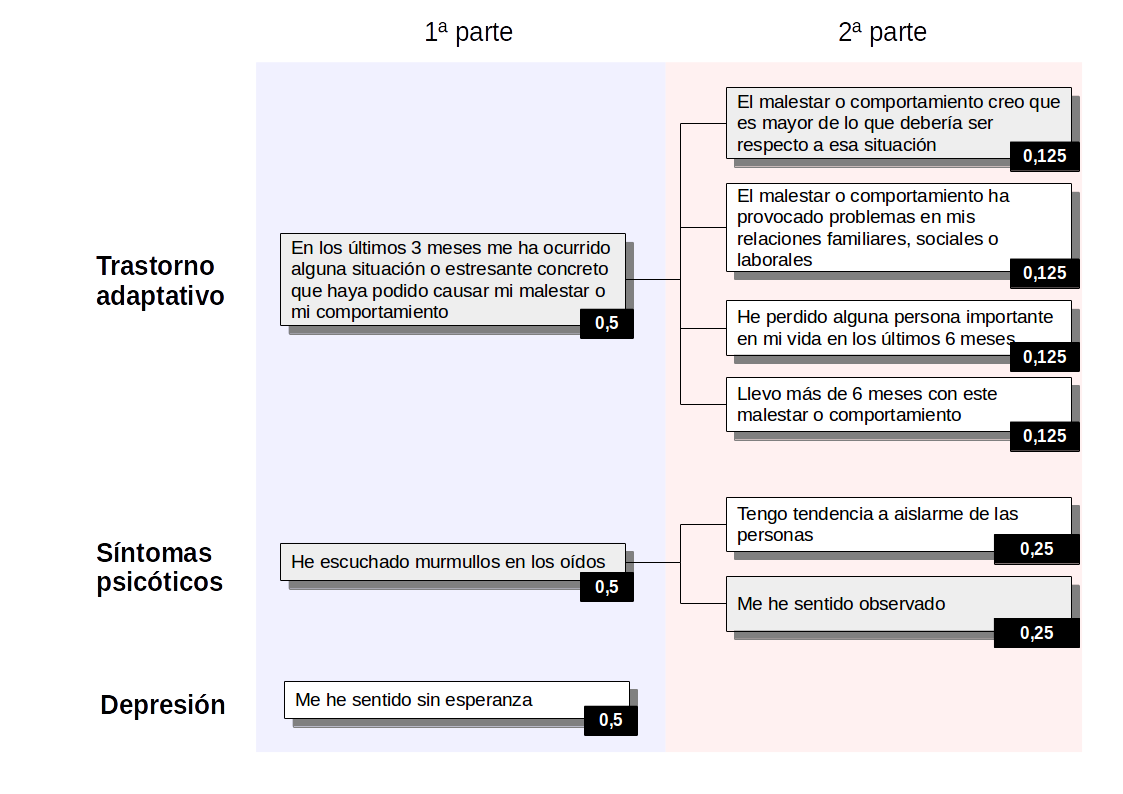
\includegraphics[width=1\textwidth]{figuras/alg_matching.png}
    \caption{Ejemplo algoritmo de \textit{matching}}
    \label{ej_alg_match}
\end{figure}	

Si el paciente marcase las preguntas que aparecen en color gris, en la segunda parte del test aparecerían el resto de preguntas de la patología en cuestión.


Tras finalizar el test, los resultados serían:

\begin{itemize}
\item Trastorno adaptativo 0,625: Se descartaría.
\item Síntomas psicóticos 0,75
\end{itemize}

%%%%%%%%%%%%%%%%%%%%%%%%%%%%%%%%%%%%%%%%%%%%%%%%%%%%%%%%%%%%%%%%%%%%%%%%%%%%%%%%%%%%%%%
%TECNOLOGÍAS UTILIZADAS%%%%%%%%%%%%%%%%%%%%%%%%%%%%%%%%%%%%%%%%%%%%%%%%%%%%%%%%%%%%%%%%
%%%%%%%%%%%%%%%%%%%%%%%%%%%%%%%%%%%%%%%%%%%%%%%%%%%%%%%%%%%%%%%%%%%%%%%%%%%%%%%%%%%%%%%

%\subsection{Tecnologías utilizadas}
%
%\subsubsection{\textit{Frameworks}}
%Un \textit{framework} es una arquitectura de software que modela las relaciones generales de las entidades del dominio, y provee una estructura y una especial metodología de trabajo, la cual extiende o utiliza las aplicaciones del dominio.
%
%
%Los frameworks involucrados en nuestro proyecto son MEAN Stack, Bootstrap y Semantic UI.
%
%\paragraph{MEAN Stack}
%Es un \textit{framework} para el desarrollo de aplicaciones, y páginas web dinámicas, basadas en JavaScript: MongoDB, ExpressJS, AngularJS y NodeJS, lo cual permite que se integren entre ellas eficazmente.
%
%
%Con MongoDB podemos almacenar nuestros documentos en formato JSON, se pueden escribir consultas en nuestro servidor ExpressJS y NodeJS, y del mismo modo, pasar esos documentos JSON a nuestro \textit{frontend} hecho con AngularJS.
%
%
%El \textit{debugging} y la administración de la base de datos se vuelven más sencillas cuando el objeto almacenado en la base de datos es idéntico al objeto que tu cliente JavaScript puede ver\cite{mongodb_blog_mean_stack}.
%
%
%Algunos de los motivos por los que escogí este \textit{framework} es por su escalabilidad, rapidez y flexibilidad, ya que permite que en un futuro sea sencillo poder adaptar la aplicación a plataformas móviles, o añadir cambios con facilidad.
%
%
%Los componentes que forman el \textit{framework} son:
%
%\begin{itemize}
%\item \textbf{MongoDB}
%MongoDB es una base de datos ágil NoSQL orientada a documentos que permite que los esquemas cambien rápidamente a medida que las aplicaciones evolucionan, proporcionando siempre la funcionalidad que los desarrolladores esperan de las bases de datos tradicionales, tales como índices secundarios, un lenguaje completo de búsquedas y consistencia. En resumen, MongoDB brinda escalabilidad, rendimiento y gran disponibilidad. \cite{mongodb}
%\item \textbf{ExpressJS}
%ExpressJS es una middleware de aplicaciones web Node.js minimalista y flexible que proporciona un conjunto sólido de características para aplicaciones web y móviles. Se trata de una API REST que utiliza métodos HTTP para obtener datos o generar operaciones sobre esos datos. \cite{expressjs}
%\item \textbf{AngularJS}
%AngularJS es un framework para construir client applications en HTML y Javascript, aunque también puede ser otro lenguaje como TypeScript que sea compilado a JavaScript. El framework posee un conjunto de librerías funcionales, y otras opcionales. \cite{angularjs_arch}
%Angular permite fácilmente construir aplicaciones web, ya que combina \textit{declarative templates}, \textit{dependency injection} y \textit{end to end tooling}, e integra buenas prácticas de programación. Las aplicaciones desarrolladas con Angular funcionan tanto para web, móvil o escritorio. \cite{angularjs_docs}
%\item \textbf{NodeJS}
%NodeJS es un entorno de ejecución para JavaScript construido con el motor de JavaScript V8 de Chrome. Node.js usa un modelo de operaciones entrada/salida sin bloqueo (asíncrono) y orientado a eventos, que lo hace liviano y eficiente, ya que nunca se bloquea. 
%Node está diseñado sin hilos, este presenta un bucle de eventos como un entorno en vez de una librería. Node simplemente ingresa el bucle de eventos después de ejecutar el script de entrada. Node sale del bucle de eventos cuando no hay más callbacks que ejecutar. \cite{nodejs_about}
%\end{itemize}
%
%
%\paragraph{Bootstrap}
%Bootstrap es un \textit{framework} de código abierto para desarrollar con HTML, CSS y JS. Contiene características como un grid responsive, docenas de componentes, JavaScript plugins, tipografía, control de formularios y capacidad de personalización.\cite{bootstrap_get}
%
%
%\paragraph{Semantic UI}
%Semantic UI es un \textit{framework} que permite a los desarrolladores contruir rápidamente sitios web, con HTML conciso, JavaScript intuitivo, y simplicando el \textit{debugging}. Semantic está diseñado de manera responsive permitiendo que la aplicación sea escalable en múltiples dispositivos. Semantic está preparado para poder asociarse con otros \textit{frameworks} como React, Angular, Meteor y Ember. \cite{semanticui_github}
%
%
%\subsection{Lenguajes de programación}




